%%%%%%%%%%%%%%%%%%%%%%%%%%%%%%%%%%%%%%%%%
% Programming/Coding Assignment
% LaTeX Template
%
% This template has been downloaded from:
% http://www.latextemplates.com
%
% Original author:
% Ted Pavlic (http://www.tedpavlic.com)
%
% Note:
% The \lipsum[#] commands throughout this template generate dummy text
% to fill the template out. These commands should all be removed when 
% writing assignment content.
%
% This template uses a Perl script as an example snippet of code, most other
% languages are also usable. Configure them in the "CODE INCLUSION 
% CONFIGURATION" section.
%
%%%%%%%%%%%%%%%%%%%%%%%%%%%%%%%%%%%%%%%%%

%----------------------------------------------------------------------------------------
%	PACKAGES AND OTHER DOCUMENT CONFIGURATIONS
%----------------------------------------------------------------------------------------

\documentclass{article}

\usepackage{fancyhdr} % Required for custom headers
\usepackage{lastpage} % Required to determine the last page for the footer
\usepackage{extramarks} % Required for headers and footers
\usepackage[usenames,dvipsnames]{color} % Required for custom colors
\usepackage{graphicx} % Required to insert images
\usepackage{listings} % Required for insertion of code
\usepackage{courier} % Required for the courier font
\usepackage{lipsum} % Used for inserting dummy 'Lorem ipsum' text into the template
\usepackage{hyperref}

% Margins
\topmargin=-0.45in
\evensidemargin=0in
\oddsidemargin=0in
\textwidth=6.5in
\textheight=9.0in
\headsep=0.25in

\linespread{1.1} % Line spacing

% Set up the header and footer
\pagestyle{fancy}
\lhead{\hmwkAuthorName} % Top left header
\chead{\hmwkClass\ (\hmwkClassInstructor\ \hmwkClassTime): \hmwkTitle} % Top center head
\rhead{\firstxmark} % Top right header
\lfoot{\lastxmark} % Bottom left footer
\cfoot{} % Bottom center footer
\rfoot{Page\ \thepage\ of\ \protect\pageref{LastPage}} % Bottom right footer
\renewcommand\headrulewidth{0.4pt} % Size of the header rule
\renewcommand\footrulewidth{0.4pt} % Size of the footer rule

\setlength\parindent{0pt} % Removes all indentation from paragraphs

%----------------------------------------------------------------------------------------
%	CODE INCLUSION CONFIGURATION
%----------------------------------------------------------------------------------------

\definecolor{MyDarkGreen}{rgb}{0.0,0.4,0.0} % This is the color used for comments
\lstloadlanguages{Perl} % Load Perl syntax for listings, for a list of other languages supported see: ftp://ftp.tex.ac.uk/tex-archive/macros/latex/contrib/listings/listings.pdf
\lstset{language=python, % Use Perl in this example
        frame=single, % Single frame around code
        basicstyle=\small\ttfamily, % Use small true type font
        keywordstyle=[1]\color{Blue}\bf, % Perl functions bold and blue
        keywordstyle=[2]\color{Purple}, % Perl function arguments purple
        keywordstyle=[3]\color{Blue}\underbar, % Custom functions underlined and blue
        identifierstyle=, % Nothing special about identifiers                                         
        commentstyle=\usefont{T1}{pcr}{m}{sl}\color{MyDarkGreen}\small, % Comments small dark green courier font
        stringstyle=\color{Purple}, % Strings are purple
        showstringspaces=false, % Don't put marks in string spaces
        tabsize=5, % 5 spaces per tab
        %
        % Put standard Perl functions not included in the default language here
        morekeywords={rand},
        %
        % Put Perl function parameters here
        morekeywords=[2]{on, off, interp},
        %
        % Put user defined functions here
        morekeywords=[3]{test},
       	%
        morecomment=[l][\color{Blue}]{...}, % Line continuation (...) like blue comment
        numbers=left, % Line numbers on left
        firstnumber=1, % Line numbers start with line 1
        numberstyle=\tiny\color{Blue}, % Line numbers are blue and small
        stepnumber=5, % Line numbers go in steps of 5
	breaklines=true
}

% Creates a new command to include a perl script, the first parameter is the filename of the script (without .pl), the second parameter is the caption
\newcommand{\pythonscript}[2]{
\begin{itemize}
\item[]\lstinputlisting[caption=#2,label=#1]{#1.py}
\end{itemize}
}

%----------------------------------------------------------------------------------------
%	DOCUMENT STRUCTURE COMMANDS
%	Skip this unless you know what you're doing
%----------------------------------------------------------------------------------------

% Header and footer for when a page split occurs within a problem environment
\newcommand{\enterProblemHeader}[1]{
\nobreak\extramarks{#1}{#1 continued on next page\ldots}\nobreak
\nobreak\extramarks{#1 (continued)}{#1 continued on next page\ldots}\nobreak
}

% Header and footer for when a page split occurs between problem environments
\newcommand{\exitProblemHeader}[1]{
\nobreak\extramarks{#1 (continued)}{#1 continued on next page\ldots}\nobreak
\nobreak\extramarks{#1}{}\nobreak
}

\setcounter{secnumdepth}{0} % Removes default section numbers
\newcounter{homeworkProblemCounter} % Creates a counter to keep track of the number of problems

\newcommand{\homeworkProblemName}{}
\newenvironment{homeworkProblem}[1][Problem \arabic{homeworkProblemCounter}]{ % Makes a new environment called homeworkProblem which takes 1 argument (custom name) but the default is "Problem #"
\stepcounter{homeworkProblemCounter} % Increase counter for number of problems
\renewcommand{\homeworkProblemName}{#1} % Assign \homeworkProblemName the name of the problem
\section{\homeworkProblemName} % Make a section in the document with the custom problem count
\enterProblemHeader{\homeworkProblemName} % Header and footer within the environment
}{
\exitProblemHeader{\homeworkProblemName} % Header and footer after the environment
}

\newcommand{\problemAnswer}[1]{ % Defines the problem answer command with the content as the only argument
\noindent\framebox[\columnwidth][c]{\begin{minipage}{0.98\columnwidth}#1\end{minipage}} % Makes the box around the problem answer and puts the content inside
}

\newcommand{\homeworkSectionName}{}
\newenvironment{homeworkSection}[1]{ % New environment for sections within homework problems, takes 1 argument - the name of the section
\renewcommand{\homeworkSectionName}{#1} % Assign \homeworkSectionName to the name of the section from the environment argument
\subsection{\homeworkSectionName} % Make a subsection with the custom name of the subsection
\enterProblemHeader{\homeworkProblemName\ [\homeworkSectionName]} % Header and footer within the environment
}{
\enterProblemHeader{\homeworkProblemName} % Header and footer after the environment
}

%----------------------------------------------------------------------------------------
%	NAME AND CLASS SECTION
%----------------------------------------------------------------------------------------

\newcommand{\hmwkTitle}{Assignment\ \#8} % Assignment title
\newcommand{\hmwkDueDate}{Friday,\ November\ 14,\ 2014} % Due date
\newcommand{\hmwkClass}{CS\ 595} % Course/class
\newcommand{\hmwkClassTime}{4:20pm} % Class/lecture time
\newcommand{\hmwkClassInstructor}{Dr Nelson} % Teacher/lecturer
\newcommand{\hmwkAuthorName}{Victor Nwala} % Your name

%----------------------------------------------------------------------------------------
%	TITLE PAGE
%----------------------------------------------------------------------------------------

\title{
\vspace{2in}
\textmd{\textbf{\hmwkClass:\ \hmwkTitle}}\\
\normalsize\vspace{0.1in}\small{Due\ on\ \hmwkDueDate}\\
\vspace{0.1in}\large{\textit{\hmwkClassInstructor\ \hmwkClassTime}}
\vspace{3in}
}

\author{\textbf{\hmwkAuthorName}}
\date{} % Insert date here if you want it to appear below your name

%----------------------------------------------------------------------------------------

\begin{document}

\maketitle

%----------------------------------------------------------------------------------------
%	TABLE OF CONTENTS
%----------------------------------------------------------------------------------------

%\setcounter{tocdepth}{1} % Uncomment this line if you don't want subsections listed in the ToC

\newpage
\tableofcontents
\newpage

%----------------------------------------------------------------------------------------
%	PROBLEM 1
%----------------------------------------------------------------------------------------

% To have just one problem per page, simply put a \clearpage after each problem

\begin{homeworkProblem}
1.  What 5 movies have the highest average ratings? Show the movies
and their ratings sorted by their average ratings.





The code sorts the result from least to highest rated movie. Their rankings are:

1) 1201|Marlene Dietrich: Shadow and Light (1996)
2) 1293|Star Kid (1997)
3) 1189|Prefontaine (1997)
4) 1653|Entertaining Angels: The Dorothy Day Story (1996)
5) 1536|Aiqing wansui (1994)
All with average ratings of 5.0






\pythonscript{ques1}{Python script solving problem 1}


\problemAnswer{
\begin{center}
Figure 1: ques1.py at work
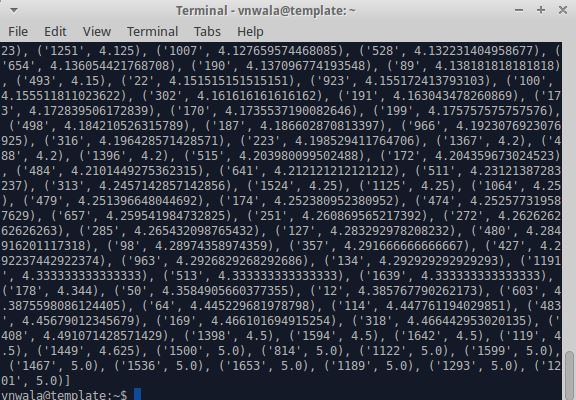
\includegraphics[width=0.75\columnwidth]{ques1} 
\end{center}

}
\end{homeworkProblem}
\newpage


%----------------------------------------------------------------------------------------
%	PROBLEM 2
%----------------------------------------------------------------------------------------

\begin{homeworkProblem}

2.  What 5 movies received the most ratings? Show the movies and
the number of ratings sorted by number of ratings.






The code sorts the result from least to most rated movie. Their rankings are:

1) 50|Star Wars (1977) with 583 ratings
2) 258|Contact (1997) with 509 ratings
3) 100|Fargo (1996)  with 508 ratings
4) 181|Return of the Jedi (1983) with 507 ratings
5) 294|Liar Liar (1997) with 485 ratings







\pythonscript{ques2}{Python script solving problem 2}


\problemAnswer{


\begin{center}
Figure 2: ques2.py at work
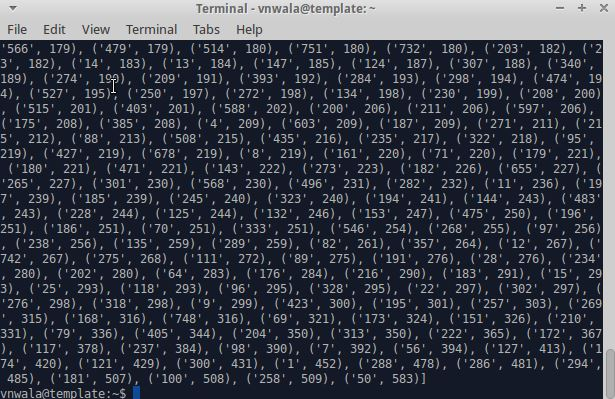
\includegraphics[width=0.75\columnwidth]{ques2} 
\end{center}


}

\end{homeworkProblem}
\newpage


%----------------------------------------------------------------------------------------
%	PROBLEM 3
%----------------------------------------------------------------------------------------

\begin{homeworkProblem}
3.  What 5 movies were rated the highest on average by women? Show
the movies and their ratings sorted by ratings.

1) 286|English Patient, The (1996) with 152 female raters
2) 50|Star Wars (1977) with 151 female raters
3) 288|Scream (1996) with 143 female raters
4) 294|Liar Liar (1997) with 141 female raters
5) 258|Contact (1997) with 137 female raters



\pythonscript{ques3}{Python script solving problem 3}

\problemAnswer{


\begin{center}
Figure 3: ques3.py at work
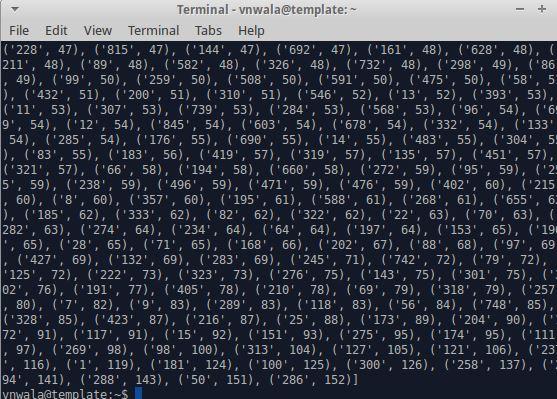
\includegraphics[width=0.75\columnwidth]{ques3} 
\end{center}


}




\end{homeworkProblem}

\newpage
%----------------------------------------------------------------------------------------
%	PROBLEM 4
%----------------------------------------------------------------------------------------

\begin{homeworkProblem}

4.  What 5 movies were rated the highest on average by men? Show
the movies and their ratings sorted by ratings.

1) 50|Star Wars (1977) with 432 male raters
2) 181|Return of the Jedi (1983) with 383 male raters
3) 100|Fargo (1996) with 383 male raters
4) 258|Contact (1997) with 372 male raters
5) 294|Liar Liar (1997) with 344 male raters



\pythonscript{ques4}{Python script solving problem 4}

\problemAnswer{


\begin{center}
Figure 4: ques4.py at work
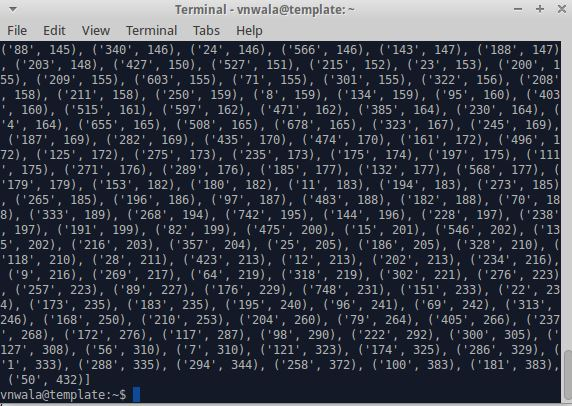
\includegraphics[width=0.75\columnwidth]{ques4} 
\end{center}


}

\end{homeworkProblem}



\newpage
%----------------------------------------------------------------------------------------
%	PROBLEM 5
%----------------------------------------------------------------------------------------

\begin{homeworkProblem}

5.  What movie received ratings most like Top Gun? Which movie
received ratings that were least like Top Gun (negative correlation)?






Some movies rated the most like like Top Gun are:


1) Mr. Smith Goes to Washington (1939)
2) (Cold Fever) (1994)
3) Young Guns II (1990)
4) Young Poisoner's Handbook, The (1995)
6) Zeus and Roxanne (1997)
7) Young Poisoner's Handbook, The (1995)
8) Out to Sea (1997)
9) Old Yeller (1957)
10) Hungarian Fairy Tale, A (1987)

\pythonscript{ques5}{Python script solving problem 5}

\problemAnswer{


\begin{center}
Figure 5: ques5.py at work
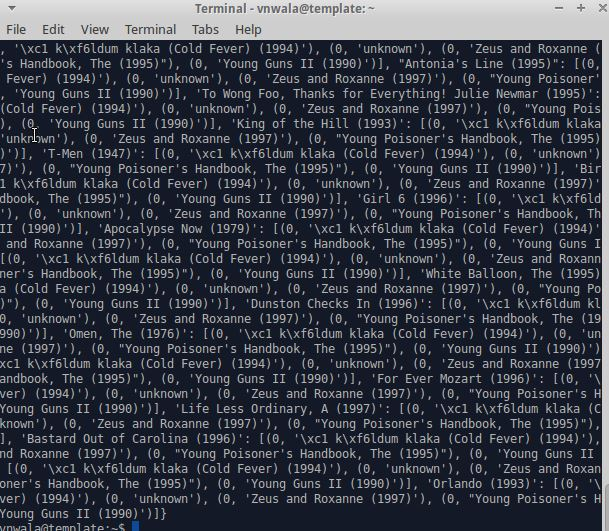
\includegraphics[width=0.75\columnwidth]{ques5} 
\end{center}


}



\end{homeworkProblem}






\newpage
%----------------------------------------------------------------------------------------
%	PROBLEM 6
%----------------------------------------------------------------------------------------

\begin{homeworkProblem}

6.  Which 5 raters rated the most films? Show the raters' IDs and
the number of films each rated.

The solution is computed in this format, rater id:number of movies rated

1) 405:737
2) 655:685
3) 13:636
4) 450:540
5) 276:518


\pythonscript{ques6}{Python script solving problem 6}

\problemAnswer{


\begin{center}
Figure 6: ques6.py at work
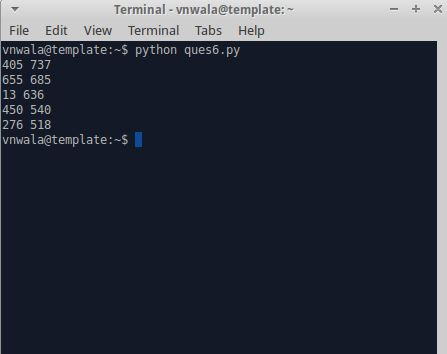
\includegraphics[width=0.75\columnwidth]{ques6} 
\end{center}


}



\end{homeworkProblem}

\newpage
%----------------------------------------------------------------------------------------
%	PROBLEM 7
%----------------------------------------------------------------------------------------

\begin{homeworkProblem}


7.  Which 5 raters most agreed with each other? Show the raters'
IDs and Pearson's r, sorted by r.

Some 5 raters that mostly agree with each other, represented by the IDs are:
'100', '105', '107', '111' and '112'


\pythonscript{ques7}{Python script solving problem 7}

\problemAnswer{


\begin{center}
Figure 7: ques7.py at work
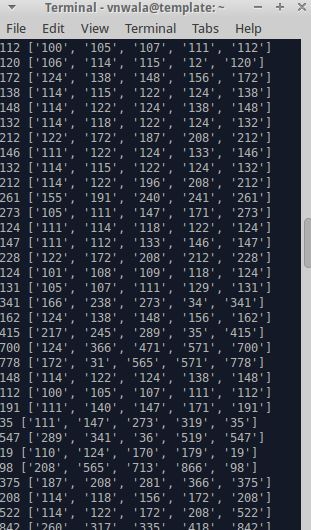
\includegraphics[width=0.75\columnwidth]{ques7} 
\end{center}


}


\end{homeworkProblem}


\newpage
%----------------------------------------------------------------------------------------
%	PROBLEM 8
%----------------------------------------------------------------------------------------

\begin{homeworkProblem}
8.  Which 5 raters most disagreed with each other (negative
correlation)? Show the raters' IDs and Pearson's r, sorted by r.

\pythonscript{ques8}{Python script solving problem 8}

\problemAnswer{


\begin{center}
Figure 8: ques8.py at work
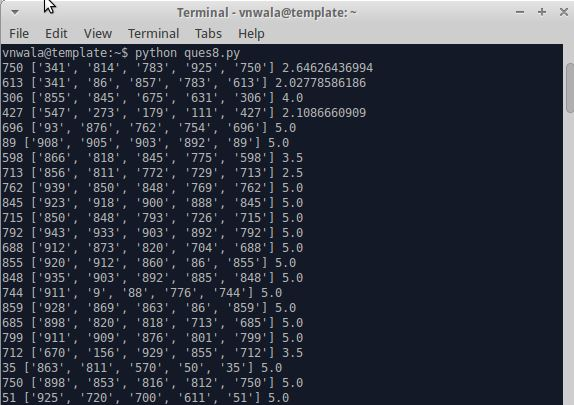
\includegraphics[width=0.75\columnwidth]{ques8} 
\end{center}


}





\end{homeworkProblem}


\newpage
%----------------------------------------------------------------------------------------
%	PROBLEM 9
%----------------------------------------------------------------------------------------

\begin{homeworkProblem}
9.  What movie was rated highest on average by men over 40? By men
under 40?





For men over 40 we have:
1) Great Day in Harlem, A (1994) 5.0
2) Two or Three Things I Know About Her (1966) 5.0
3) Aparajito (1956) 5.0
4) Strawberry and Chocolate (Fresa y chocolate) (1993) 5.0
5) Little Princess, The (1939) 5.0




For men under 40 we have:
1) Entertaining Angels: The Dorothy Day Story (1996) 5.0
2) Letter From Death Row, A (1998) 5.0
3) Hugo Pool (1997) 5.0
4) Leading Man, The (1996) 5.0
5) Quiet Room, The (1996) 5.0




\pythonscript{ques9}{Python script solving problem 9}

\problemAnswer{


\begin{center}
Figure 9: ques9.py at work
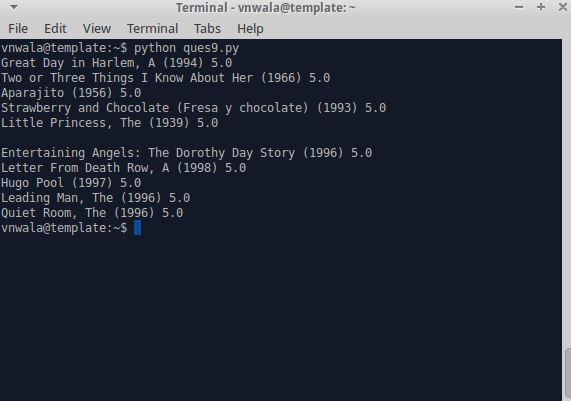
\includegraphics[width=0.75\columnwidth]{ques9} 
\end{center}


}



\end{homeworkProblem}




\newpage
%----------------------------------------------------------------------------------------
%	PROBLEM 10
%----------------------------------------------------------------------------------------

\begin{homeworkProblem}

10. What movie was rated highest on average by women over 40? By
women under 40?






For women over 40 we have:

1) In the Bleak Midwinter (1995) 5.0
2) Foreign Correspondent (1940) 5.0
3) Swept from the Sea (1997) 5.0
4) Great Dictator, The (1940) 5.0
5) Balto (1995) 5.0




 

For women under 40 we have:
1) Nico Icon (1995) 5.0
2) Backbeat (1993) 5.0
3) Umbrellas of Cherbourg, The (Parapluies de Cherbourg, Les) (1964) 5.0
4) Everest (1998) 5.0
5) Someone Else's America (1995) 5.0


\pythonscript{ques10}{Python script solving problem 10}

\problemAnswer{


\begin{center}
Figure 10: ques10.py at work
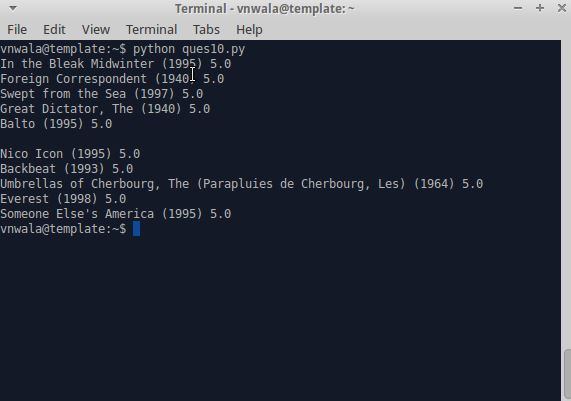
\includegraphics[width=0.75\columnwidth]{ques10} 
\end{center}


}


\end{homeworkProblem}

\section{Conclusion}
To conclude, I should state that Alexander Nwala was a huge contributor for my answers from question 6 to 10, so those answers will in some or most cases have the same syntatic and functional properties similar to his code. Some questions were answered in part, depending on what I was able to do.

\newpage
%------------------------------------------------------------------
%  Bibilography
%------------------------------------------------------------------
\bibliographystyle{plain}
\bibliography{assignment_8}
\cite{*}
%----------------------------------------------------------------------------------------

\end{document}
